\section{Introducción}


\begin{frame}{Qubits}
    \begin{center}
        ``\textbf{Dinámica} efectiva de un sistema de N \textbf{qubits}''
    \end{center}
    \pause
    \begin{columns}
        \begin{column}{0.5\textwidth}
            \begin{center}
                Un qubit es un sistema cuántico de dos estados.
                \pause
                Todo qubit se puede escribir como
                \begin{equation}
                    \ket{\psi}=\alpha\ket{0}+\beta\ket{1}.\nonumber
                \end{equation}
                \pause
                Por convención usamos los eigenestados del operador $\pauli{3}$.
                \begin{align}
                    \ket{0} & & \text{y} & & \ket{1}. \nonumber
                \end{align} 
            \end{center}
        \end{column}
        \pause
        \begin{column}{0.5\textwidth}
            La evolución de un sistema cuántico descrito por $\ket{\psi}$ está dada por
            \begin{equation}
                \rmi\hbar\frac{d}{dt}\ket{\psi(t)}=H\ket{\psi(t)}.\nonumber
            \end{equation}
            \pause
            Cuya solución es una evolución unitaria $U(t,t_{0})=e^{-\rmi H(t-t_{0})/\hbar}$
            \begin{align}
                \ket{\psi(t)}=U(t,t_{0})\ket{\psi(t_{0})} \rlap{.}\nonumber
            \end{align}
        \end{column}
    \end{columns}
\end{frame}

\begin{frame}{Parametrización de un qubit}
    \begin{columns}
        \begin{column}{0.5\textwidth}
            Un qubit $\ket{\psi}\in\hilbert_{2}$ arbitrario
            \begin{equation}
                \ket{\psi}=\alpha\ket{0}+\beta\ket{1},\nonumber
            \end{equation}
            \pause
            se puede reescribir como:
            \begin{equation}
                \ket{\psi}=\cos(\frac{\theta}{2})\ket{0}+e^{\rmi\varphi}\sin(\frac{\theta}{2})\ket{1}.\nonumber
            \end{equation}
        \end{column}
        \begin{column}{0.5\textwidth}
            \centering
            \BlochSphere
        \end{column}
    \end{columns}
\end{frame}



\begin{frame}{Efectiva}
    \begin{center}
        ``Dinámica \textbf{efectiva} de un sistema de N qubits''
    \end{center}
    \pause
    \begin{columns}
        \begin{column}{0.5\textwidth}
            \begin{center}
                Dinámica \textbf{efectiva}\\
                \pause
                $\downarrow$\\
                Dinámica {\tiny(que emerge de una descripción)} \textbf{efectiva}
            \end{center}
            \pause
            Aquí, 
            \begin{center}
                \textit{efectiva}$\iff$\textit{gruesa}.
            \end{center}
        \end{column}
        \pause
        \begin{column}{0.5\textwidth}
            La descripción gruesa de un sistema puede ser resultado de
            \begin{itemize}
                \item Aparato de medición imperfecto
                \item Descarte de grados de libertad del sistema
            \end{itemize}
        \end{column}
    \end{columns}
\end{frame}

\begin{frame}{Modelos de grano grueso}
    \begin{center}
        Una descripción de grano grueso es aquella que no toma en cuenta todos los detalles de un sistema o fenómeno.
    \end{center}
    \pause
    \begin{columns}
        \begin{column}{0.5\textwidth}
            \begin{center}
                Variables termodinámicas\\
                $\downarrow$\\
                Descripción efectiva\\
                \pause
                \begin{equation}
                    T=\frac{1}{k_\text{B}}\frac{2}{3}\expval{E_{\text{cin}}}.\nonumber
                \end{equation}
            \end{center}
        \end{column}
        \begin{column}{0.5\textwidth}
            \begin{figure}
                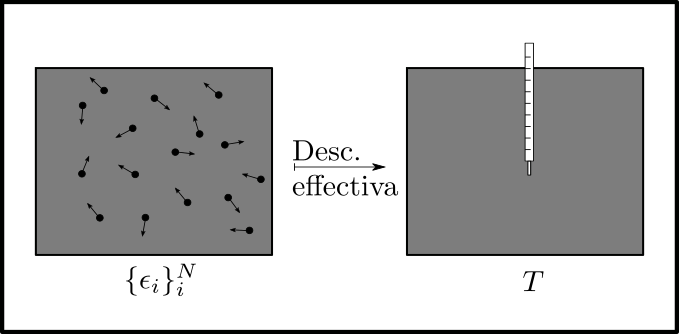
\includegraphics[width=1\textwidth]{figures/CGT.png}
            \end{figure}
        \end{column}
    \end{columns}
\end{frame}

\subsection{El operador de densidad}

\begin{frame}{Mezclas estadísticas}
    \begin{columns}
        \begin{column}{0.5\textwidth}
            Los vectores de estado contienen probabilidad cuántica:
            \begin{equation}
                \ket{\psi}=\frac{1}{\sqrt{2}}(\ket{0}+\ket{1}),\nonumber
            \end{equation}
            \pause
            pero no el segundo tipo de probabilidad: la asociada a la ignorancia.
        \end{column}
        \pause
        \begin{column}{0.5\textwidth}
            Un sistema del que se sabe se halla en el estado $\ket{\varphi_{j}}$ con probabilidad $p_{j}$.\\
            \vspace{0.2cm}
            \pause
            De este sistema se halla en un estado de \textit{mezcla estadística}.\\
            \vspace{0.2cm}
            \pause
            Es descrito por el operador de densidad
            \begin{equation}
                \rho=\sum_{j}p_{j}\dyad{\varphi_{j}}.\nonumber
            \end{equation}
        \end{column}
    \end{columns}
\end{frame}

\begin{frame}{Parametrización}
    \begin{columns}
        \begin{column}{0.5\textwidth}
            Una base hermítica permite parametrizar a una matriz de densidad a través del producto punto de Hilbert-Schmidt
            \begin{equation}
                \rho=\frac{1}{2}\qty(\Id_{2}\Tr(\rho)+\sum_{k=1}^{3}\Tr(\rho\pauli{k})\pauli{k}).\nonumber
            \end{equation}
            \pause
            El vector de Bloch es
            \begin{equation}
                \vec{r}_{\rho}=\begin{pmatrix}
                    \Tr(\rho\pauli{x})\\
                    \Tr(\rho\pauli{y})\\
                    \Tr(\rho\pauli{z})
                \end{pmatrix}\nonumber
            \end{equation}
        \end{column}
        \pause
        \begin{column}{0.5\textwidth}
            \centering
            \BlochSphereDensity
        \end{column}
    \end{columns}
\end{frame}


\begin{frame}{Sistemas multipartitos}
    \begin{center}
        ``Dinámica efectiva de un sistema de \textbf{N} qubits''
    \end{center}
    \pause
    \begin{columns}
        \begin{column}{0.5\textwidth}
            \begin{equation}
                \hilbert_{\text{bi}}=\hilbert_{2}\otimes\hilbert_{2}.\nonumber
            \end{equation} \pause
            La dimensión cumple
           \begin{equation}
               \text{dim}(\hilbert_{\text{bi}})=\text{dim}(\hilbert_{2})\text{dim}(\hilbert_{2}).\nonumber
           \end{equation}
           \pause
           ¿Qué sucede si únicamente nos es relevante el estado de una partícula?
        \end{column}
        \pause
        \begin{column}{0.5\textwidth}
             Si $\rho_{\text{bi}}$ describe dos qubits A y B, \pause
            \begin{equation}
                \rho^{A}=\Tr_{B}(\rho_{\text{bi}}),\nonumber
            \end{equation}
            donde $\Tr_{B}$ es la traza parcial respecto al qubit $B$.\\
            \pause
            \begin{center}
                ¿Y la evolución?
            \end{center}
        \end{column}
    \end{columns}
\end{frame}

\begin{frame}{Evolución abierta}
    Supóngase que el sistema de interés está acoplado a un \textit{entorno}: $\rho(0)=\rho_{S}(0)\otimes\rho_{E}$
    \vspace*{0.3cm}
    \begin{columns}
        \begin{column}{0.5\textwidth}
            El sistema completo evoluciona de forma unitaria.\begin{equation}
                \rmi\hbar\frac{d}{d t} \rho(t)=[H,\rho(t)].\nonumber
            \end{equation}\pause
            Para hallar la dinámica del sistema de interés hay que trazar:
            \begin{align}
                \rmi\hbar\frac{d}{d t} \rho_{S}(t)=\Tr_{E}([H,\rho(t)])\rlap{,}\nonumber
            \end{align}
        \end{column}
        \pause
        \begin{column}{0.5\textwidth}
            \begin{equation}
                \rho_{S}(t)=\mcE_{t}(\rho_{S}(0)).\nonumber
            \end{equation}\pause
            \begin{equation}
                \mcE_{t}(\rho_{S}(0))=\Tr_{E}\qty[U(t,0)\left(\rho_{S}(0)\otimes\rho_{E}\right)U^{\dag}(t,0)],\nonumber
            \end{equation}\pause
            Es un canal cuántico y\pause
            \begin{equation}
                \mcE(\rho)=\sum_{k}A_{k}\rho A^{\dagger}_{k}\nonumber
            \end{equation}\pause
            es su representación en suma de operadores de Kraus.
        \end{column}
    \end{columns}
\end{frame}

\begin{frame}{Canal de desfasamiento}
    El \textit{canal de desfasamiento} tiene operadores de Kraus $\{\sqrt{p}\Id,\sqrt{(1-p)}\pauli{3}\}$. Su efecto sobre un estado $\rho$ es
    \begin{equation}
        \rho\mapsto p\rho+(1-p)\pauli{3}\rho\pauli{3}.\nonumber
    \end{equation}
    \begin{figure}
        \centering
        \begin{subfigure}{0.45\textwidth}
            \centering
            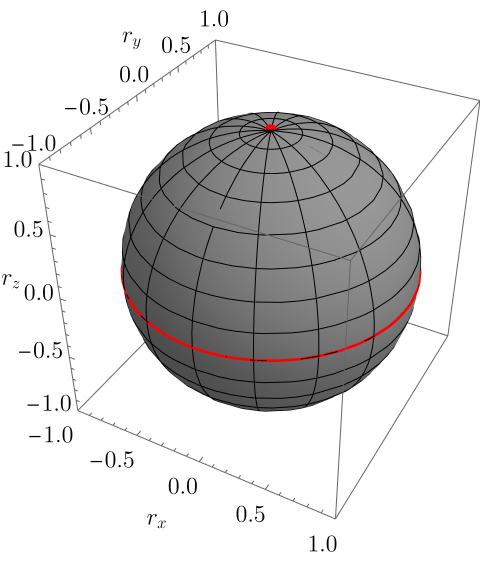
\includegraphics[width=0.5\textwidth]{figures/whole_sphere.png}
        \end{subfigure}
        \begin{subfigure}{0.45\textwidth}
            \centering
            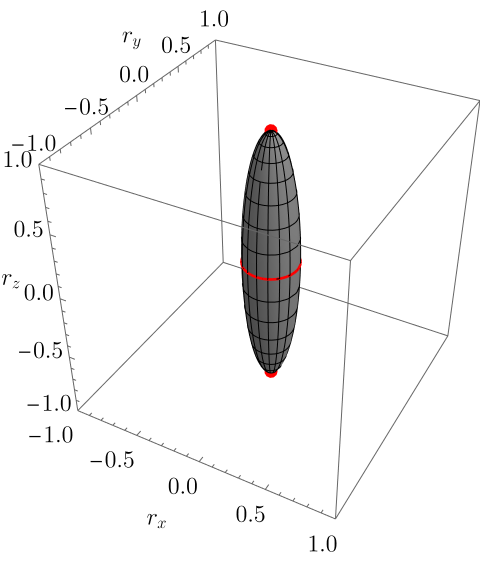
\includegraphics[width=0.5\textwidth]{figures/dephased.png}
        \end{subfigure}
    \end{figure}
\end{frame}

\begin{frame}{Canal de bitflip}
    El \textit{canal de bitflip} tiene operadores de Kraus $\{\sqrt{p}\Id,\sqrt{(1-p)}\pauli{1}\}$. Su efecto es el de reducir la magnitud de las componentes de $\pauli{2}$ y $\pauli{3}$ por un factor de $2p-1$.
    \begin{figure}
        \centering
        \begin{subfigure}{0.45\textwidth}
            \centering
            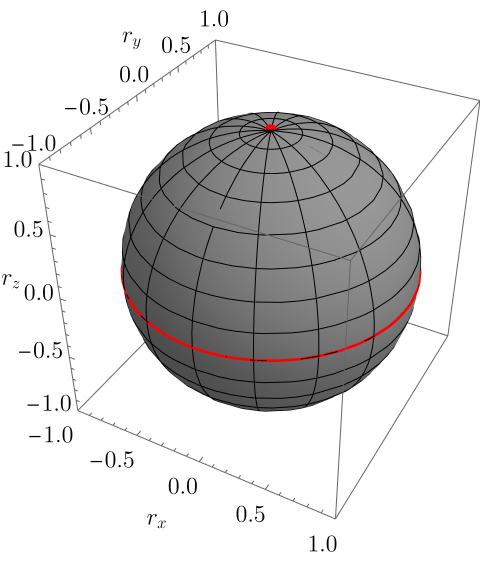
\includegraphics[width=0.5\textwidth]{figures/whole_sphere.png}
        \end{subfigure}
        \begin{subfigure}{0.45\textwidth}
            \centering
            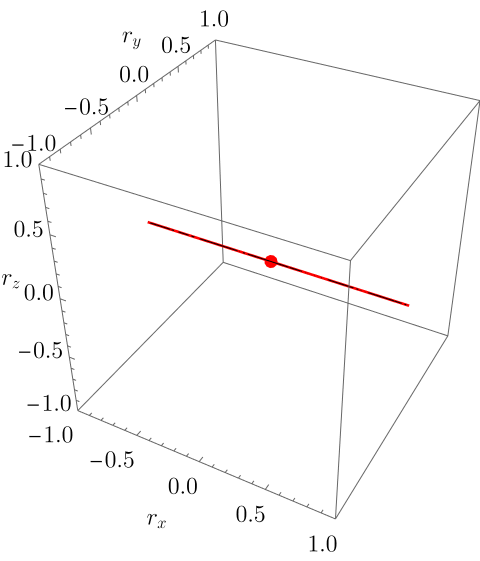
\includegraphics[width=0.5\textwidth]{figures/bitflip.png}
        \end{subfigure}
    \end{figure}
\end{frame}

\begin{frame}{Canal de despolarización}
    Finalmente, el \textit{canal de despolarización} se define mediante
    \begin{equation}
        \rho\mapsto p\frac{1}{2}\Id+(1-p)\rho\nonumber.
    \end{equation}
    \begin{figure}
        \centering
        \begin{subfigure}{0.45\textwidth}
            \centering
            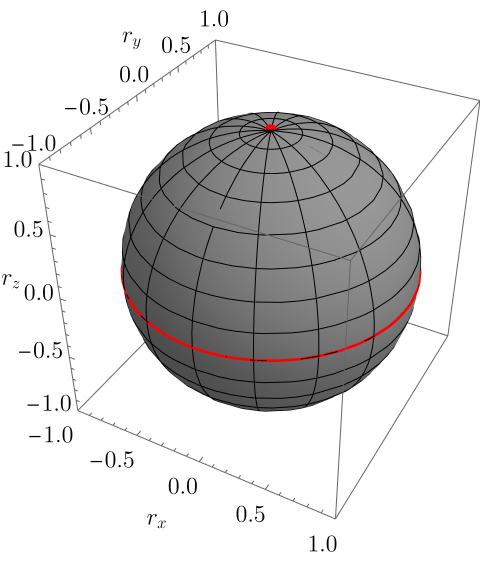
\includegraphics[width=0.5\textwidth]{figures/whole_sphere.png}
        \end{subfigure}
        \begin{subfigure}{0.45\textwidth}
            \centering
            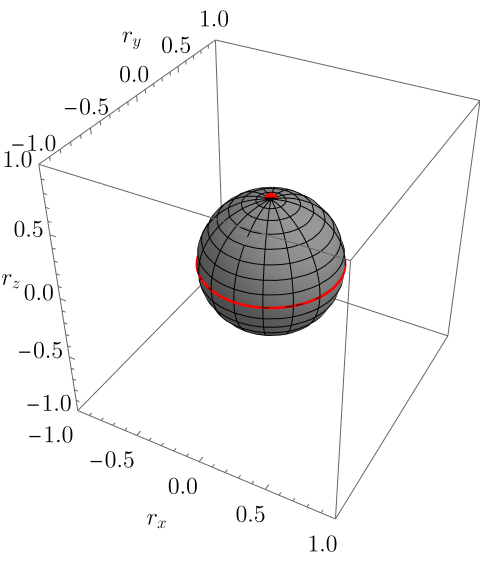
\includegraphics[width=0.5\textwidth]{figures/depol.png}
        \end{subfigure}
    \end{figure}
\end{frame}

\begin{frame}{El problema}
    \begin{center}
        ``Dinámica efectiva de un sistema de N qubits''
    \end{center}
    \begin{columns}
        \begin{column}{0.5\textwidth}
            \begin{displaymath}
                \xymatrix{
                  {\rho_{\ef}(0)} \ar[rr]^{\text{?}}
                  && {\rho_{\ef}(t)}\\
                  {\varrho_{\text{?}}(0)} \ar[rr]^{\mcE_{t}} \ar[u]^{\mcC}
                  && {\varrho_{\text{?}}(t)} \ar[u]^{\mcC}
                }
              \end{displaymath}
        \end{column}
        \pause
        \begin{column}{0.5\textwidth}
            \begin{displaymath}
                \xymatrix{
                  {\rho_{\ef}(0)} \ar[rr]^{\Gamma} \ar[d]^{\mcA}
                  && {\rho_{\ef}(t)}\\
                  {\varrho(0)} \ar[rr]^{\mcE_{t}}
                  && {\varrho(t)} \ar[u]^{\mcC}
                }
              \end{displaymath}
              \pause
        \end{column}
    \end{columns}
    \begin{center}
        ``Utilizando el Principio de Máxima Entropía''
    \end{center}
\end{frame}

\subsection{Entropía e información}

\begin{frame}{Información clásica}
    \begin{columns}
        \begin{column}{0.5\textwidth}
            Cantidad de información $\propto$ probabilidad
            \begin{itemize}
                \item ``No cayó 6''$\rightarrow$poca información
                \item ``Cayó 6''$\rightarrow$más información
            \end{itemize}
        \end{column}
        \begin{column}{0.5\textwidth}
            Conocer el resultado de un evento que ocurre con probabilidad $p=1$ no transmite ninguna información. Si a cada valor de $X$ se le puede asociar una cantidad de información, entonces debe poder calcularse la cantidad de información promedio: esta es la medida que buscaba Shannon.
        \end{column}
    \end{columns}
\end{frame}

\begin{frame}{Entropía de Shannon}
    \begin{columns}
        \begin{column}{0.5\textwidth}
            La entropía de Shannon $S_{\text{S}}$ es una medida \textit{incertidumbre} o \textit{información}.
            \pause
            \begin{enumerate}
                \item $S_{\text{S}}(p)$ debe ser continua en $p$. \pause
                \item $S_{\text{S}}(p)$ debe ser una función creciente, monotónica de $n$ cuando $p_{j}=\frac{1}{n}$. \pause
                \item Si $X$ e $Y$ son procesos independientes, $S_{\text{S}}(p_{X}(x_{j})p_{Y}(y_{l}))=S_{\text{S}}(p_{X}(x_{j}))+S_{\text{S}}(p_{Y}(y_{l}))$.
            \end{enumerate}
        \end{column}
        \pause
        \begin{column}{0.5\textwidth}
            Claude Shannon demostró 
            \begin{equation}
                S_{\text{S}}=-k\sum_{j}p(x_{j})\log{p(x_{j})}.\nonumber
            \end{equation}
            \pause
            Fue a través de discusiones con von Neumann que Shannon descubrió que su medida ya era ampliamente utilizada en física, y que llevaba el nombre de \textit{entropía}.   
        \end{column}
    \end{columns}
\end{frame}

\begin{frame}{Entropía de Shannon}
    \begin{columns}
        \begin{column}{0.5\textwidth}
            Retomando la idea del dado bien balanceado, como no es posible tener ningún tipo de seguridad sobre el resultado de un tiro, la incertidumbre (la entropía) es máxima.

            \pause

            En teoría de información clásica, la entropía de Shannon se suele utilizar como la cantidad promedio de bits requerida para trasmitir un mensaje.

        \end{column}
        \pause
        \begin{column}{0.5\textwidth}
            ABCD $00$, $01$, $10$, y $11$ $S_{S}=2$

            \pause

            Si, en cambio, las probabilidades de que aparezca cada uno de los caracteres son $p(A)=\frac{1}{2}$, $p(B)=\frac{1}{4}$, $p(C)=\frac{1}{8}$, $p(D)=\frac{1}{8}$. En este caso, una codificación posible, tal que no haya ambigüedad en la cadena de bits, es $A \rightarrow 0$, $B\rightarrow 10$, $C\rightarrow 110$, $D\rightarrow 111$. Nótese que ahora solo se requiere un bit para transmitir la letra más común. Pues bien, si se calcula la entropía de Shannon, se encuentra que cada letra requerirá $1.75$ bits para ser transmitida


        \end{column}
    \end{columns}
\end{frame}


\subsection{El principio de Máxima Entropía}

\begin{frame}{El PME clásico}
    \begin{columns}
        \begin{column}{0.5\textwidth}
            \Pisymbol{dice3d}{102}
            {\usefont{U}{dice3d}{m}{n}6a 2b 3d}
            No hay forma de saber.
            $p(\epsdice{5})=0.5$ y $p(\epsdice{2})=0.5$
            O todo igual (maximiza la entropía)
        \end{column}
        \begin{column}{0.5\textwidth}
            El principio de máxima entropía fue introducido por E. T. Jaynes en 1957.
            Jaynes afirma que la distribución de probabilidad que maximice la entropía es la estimación menos sesgada que se puede hacer.
        \end{column}
    \end{columns}
\end{frame}

\begin{frame}{El PME clásico}
    \begin{columns}
        \begin{column}{0.5\textwidth}
            Sean $x_{j}$ los valores de $X$, $f_{k}$, funciones de valor esperado conocido. La información accesible:
            \begin{equation}
            \expval{f_{l}(x)}=\sum_{j}p(x_{j})f_{l}(x_{j}).\nonumber
            \end{equation}
            Maximizamos la entropía usando multiplicadores de Lagrange:
            \begin{equation}
                \mcL=-S_{\text{S}}(p)+\sum_{l}\lambda_{l}\qty(\sum_{j}p(x_{j})f_{l}(x_{j})-\expval{f_{l}(x)})+\mu\qty(\sum_{j}p(x_{j})-1).\nonumber
            \end{equation}
            La solución a cada componente
            \begin{equation}
                p(x_{j})=\exp[-(1+\frac{\mu}{k})-\frac{1}{k}\sum_{l}\lambda_{l}f_{l}(x_{j})].\nonumber
            \end{equation}
        \end{column}
        \begin{column}{0.5\textwidth}
            Notar que
            \begin{equation}
                \frac{1}{e^{-(1+\mu)}}=\sum_{j}\exp[-\frac{1}{k}\sum_{l}\lambda_{l}f_{l}(x_{j})].\nonumber
            \end{equation}
            La función de partición,
            \begin{equation}
                Z=\sum_{j}\exp[-\frac{1}{k}\sum_{l}\lambda_{l}f_{l}(x_{j})],\nonumber
            \end{equation}
            La distribución de probabilidad que maximiza la entropía: 
            \begin{equation}
                p(x_{j})=\frac{1}{Z}\exp[-\frac{1}{k}\sum_{l}\lambda_{l}f_{l}(x_{j})].\nonumber
            \end{equation}
        \end{column}
    \end{columns}
\end{frame}

\begin{frame}{El PME cuántico}
    \begin{columns}
        \begin{column}{0.5\textwidth}
            Utilizamos la entropía de von Neumann:
            \begin{equation}
                S=
            \end{equation}
            Sean $\rho$ $H$ tales que $[\rho,H]=0$. La entropía de von Neumann:
            \begin{equation}
                S_{\text{N}}=-\sum_{k}\eta_{k}\log{\eta_{k}}.\nonumber
            \end{equation}
        \end{column}
        \begin{column}{0.5\textwidth}
            Para maximizarla:
            \begin{equation}
                \mcL=\sum_{k}\eta_{k}\log{\eta_{k}}+\lambda_{0}\qty(\sum_{k}\eta_{k}-1)+\lambda_{1}\qty(\sum_{k}\eta_{k}E_{k}-\expval{H}),\nonumber
            \end{equation}
            cuyas soluciones son
            \begin{equation}
                \eta_{k}=-e^{(\lambda_{0}+1+\lambda_{1}E_{k})}.\nonumber
            \end{equation}
        \end{column}
    \end{columns}
\end{frame}

\begin{frame}{El PME cuántico}
   \begin{columns}
    \begin{column}{0.5\textwidth}
        Como $\sum_{k}\eta_{k}=1$, podemos definir a la función de partición notando que
        \begin{equation}
            e^{1+\lambda_{0}}=\sum_{k}e^{-\lambda_{1}E_{k}}.\nonumber
        \end{equation}
Así que la expresión de los eigenvalores del estado $\rho$ que maximiza a la entropía sujeto a la condición $\expval{H}=\sum_{k}\eta_{k}E_{k}=E$ en términos de los eigenvalores de $H$, $E_{k}$ es
\begin{equation}
\eta_{k}=\frac{1}{Z}e^{-\lambda E_{k}}.\nonumber
\end{equation}
    \end{column}
    \begin{column}{0.5\textwidth}
Utilizando notación de Dirac, $\rho=\sum_{k}\eta_{k}\dyad{e_{k}}$, podemos hallar el resultado independiente de la elección de la base:
\begin{equation}
    \rho=\frac{1}{Z}e^{-\lambda H}.
\end{equation}
Este resultado es fácilmente generalizable al caso en que contemos con un  conjunto $\{A_{j}\}_{j}$ de $N$ observables tales que $[A_{j},\rho]=0$, de los que conozcamos sus valores esperados. En general, la expresión del estado de máxima entropía es
\begin{equation}\label{eq:GeneralMaxEnt}
    \rho=\frac{1}{Z}e^{-\sum_{k}\lambda_{k} A_{k}}.
\end{equation}
    \end{column}
   \end{columns}
\end{frame}


\begin{frame}{El problema}
    \begin{center}
        ``Dinámica efectiva de un sistema de N qubits\\
        Utilizando el Principio de Máxima Entropía''
    \end{center}
\end{frame}